% 5_resultados_discussao.tex
\chapter{RESULTADOS E DISCUSSÃO}

\section[SIMULAÇÕES DAS PROPRIEDADES ESTRUTURAIS E MORFLÓGICAS DO ZnWO4]{SIMULAÇÕES DAS PROPRIEDADES ESTRUTURAIS E MORFLÓGICAS DO ZnWO$_4$}

\subsection{Otimização da estrutura interna}

Os parametros ENCUT e o \textit{k-points} são parametros cruciais em cálculos de DFT, pois influenciam diretamente a precisão dos resultados e o custo computacional. Sendo assim, é necessário realizar uma série de cálculos variando esses parametros para encontrar os valores ótimos que garantam um equilíbrio entre precisão e eficiência computacional. Esses resultados estão expostos na Figura \ref{fig:convergencia_encut_kpoints}.

\FloatBarrier
\begin{figure}[!htbp]
    \caption{Gráfico de convergência da energia total do sistema em função dos parâmetros ENCUT e \textit{k-points}.}
    \label{fig:convergencia_encut_kpoints}
    \centering
    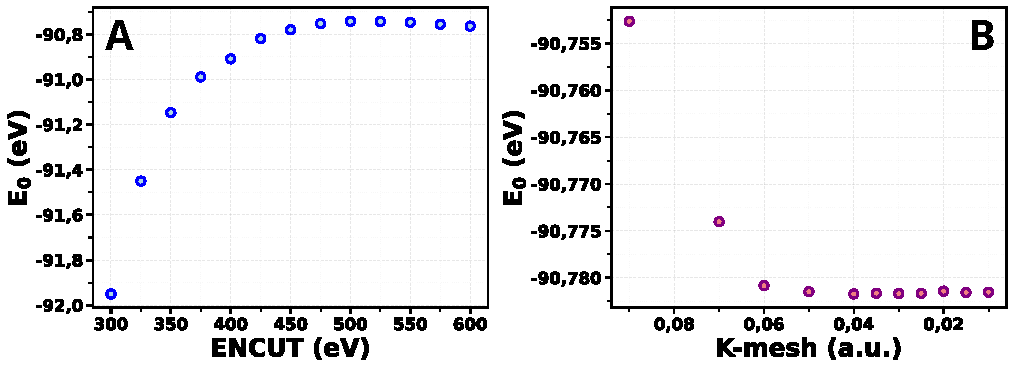
\includegraphics[width=1.0\textwidth]{figuras/graficos/convergencia_encut_kpoints.pdf}
    \fonte{Elaborada pelo autor.}
\end{figure}
\FloatBarrier

Primeiramente para a otimização do sistema foi realizada a determinação do ENCUT mínimo do sistema, que define o limite da energia cinética das funções de ondas planas que contribuirão na descrição da função de onda do sistema e com isso determinação da energia total do sistema (E$_0$). Esse parametro é de extrema importancia para descriçãoda E$_0$ e também não usar utilizar um número excessivo de funções de base que não aumentar significativamente a precisão do resultado e aumetaram o tempo de calculo, visto que acima de um valor limite a energia total do sistema tende a convergir para um valor limite. Sendo assim foram feitos calculos de relaxação do \textit{bulk} de ZnWO$_4$ variando o ENCUT de 300 a 600 eV. A partir dos resultados apresentados na Figura \ref{fig:convergencia_encut_kpoints} A observa-se que o E$_0$ do sistema converge para um valor limite a partir de um ENCUT de 450 eV, portanto esse valor foi escolhido para os cálculos subsequentes. A partir desse resultado realizou-se a determinação do número ótimo de \textit{k-points} para a amostragem da zona de Brillouin do sistema. Foram realizados cálculos variando a densidade da malha de \textit{k-points} (K-MESH) com o auxílio do \textit{vaspkit} foi gerado os \textit{k-points}, a densidade da malha foi variada de 0,01 a 0,09. A partir dos resultados apresentados na Figura \ref{fig:convergencia_encut_kpoints}B observa-se que o E$_0$ do sistema converge para um valor limite a partir de uma malha de densidade 0.04, que corresponde aos \textit{k-points} de 5x4x5, portanto esse valor foi escolhido para os cálculos subsequentes.

Feita essa otimização inicial dos parâmetros de cálculo, foi realizado um estudo do funcional de troca e correlação mais adequado para descrever o sistema, para isso foi utilizada a entalpia de formação do material como parametro de comparação. Foram testados os funcionais GGA do tipo PBE (usado até o momento), PBE revisado por Zhang e Yang (revPBE) \cite{zhang1998comment} e PBE revisado para sólidos e superfícies (PBEsol) \cite{perdew2008restoring} e PBE revisado Hammer \textit{et. al.} (RPBE) \cite{hammer1999improved} que tem como objetivo de aprimorar a descrição de energia de adsorção. A Tabela \ref{tab:entalpia_formaçao} apresenta os valores de entalpia obtidos para cada funcional testado, comparados com o valor experimental de -12,78 eV disponível na literatura \cite{dellien1976chromium}.

\FloatBarrier
\begin{table}[!htbp]
\centering
\caption{Valores de entalpia de formação do ZnWO$_4$ obtidos com diferentes funcionais de troca e correlação comparados com o valor experimental.}
\label{tab:entalpia_formaçao}
\begin{tabular}{lcc}
\hline
\textbf{Funcional} & \textbf{Entalpia de Formação (eV mol$^{-1}$)} & \textbf{Erro (\%)}
\\ \hline
PBE & -11,518 &  9,870 \\
revPBE & -10,556 & 17,40 \\
PBEsol & -11,977 & 6,280 \\
RPBE & -10,512 & 17,74 \\
Experimental \cite{dellien1976chromium} & -12,78  & - \\
\hline
\end{tabular}
\end{table}
\FloatBarrier

A partir dos resultados apresentados na Tabela \ref{tab:entalpia_formaçao} observa-se que o funcional GGA-PBEsol apresentou os valores de valor de entalpia de formação mais próximos dos valores experimentais, com um erro percentual de aproximadamente 5,86\%. Portanto, esse funcional foi escolhido para os cálculos subsequentes. 

Para terminar a otimização das estrutura do ZnWO$_4$ foi realizados calculos variando o fator de escala dos parametros de rede a fim de determinar a estrutura de mínima energia do sistema. Para isso foi feito um primeiro estudo variando o fator de escala de 0,800 a 1,300, a fim de obter uma estimativa inicial dos parametros de rede ótimos. A partir desse resultado foi realizado um segundo estudo mais refinado variando o fator de escala de 0,960 a 1,020. Os resultados desses cálculos estão apresentados na Figura \ref{fig:curva_fit_birch}.

\FloatBarrier
\begin{figure}[!htbp]
    \caption{Curva de Energia total (E$_0$) versus volume (V) do ZnWO$_4$ obtida a partir variação do fator de escala dos parametros de rede.}
    \label{fig:curva_fit_birch}
    \centering
    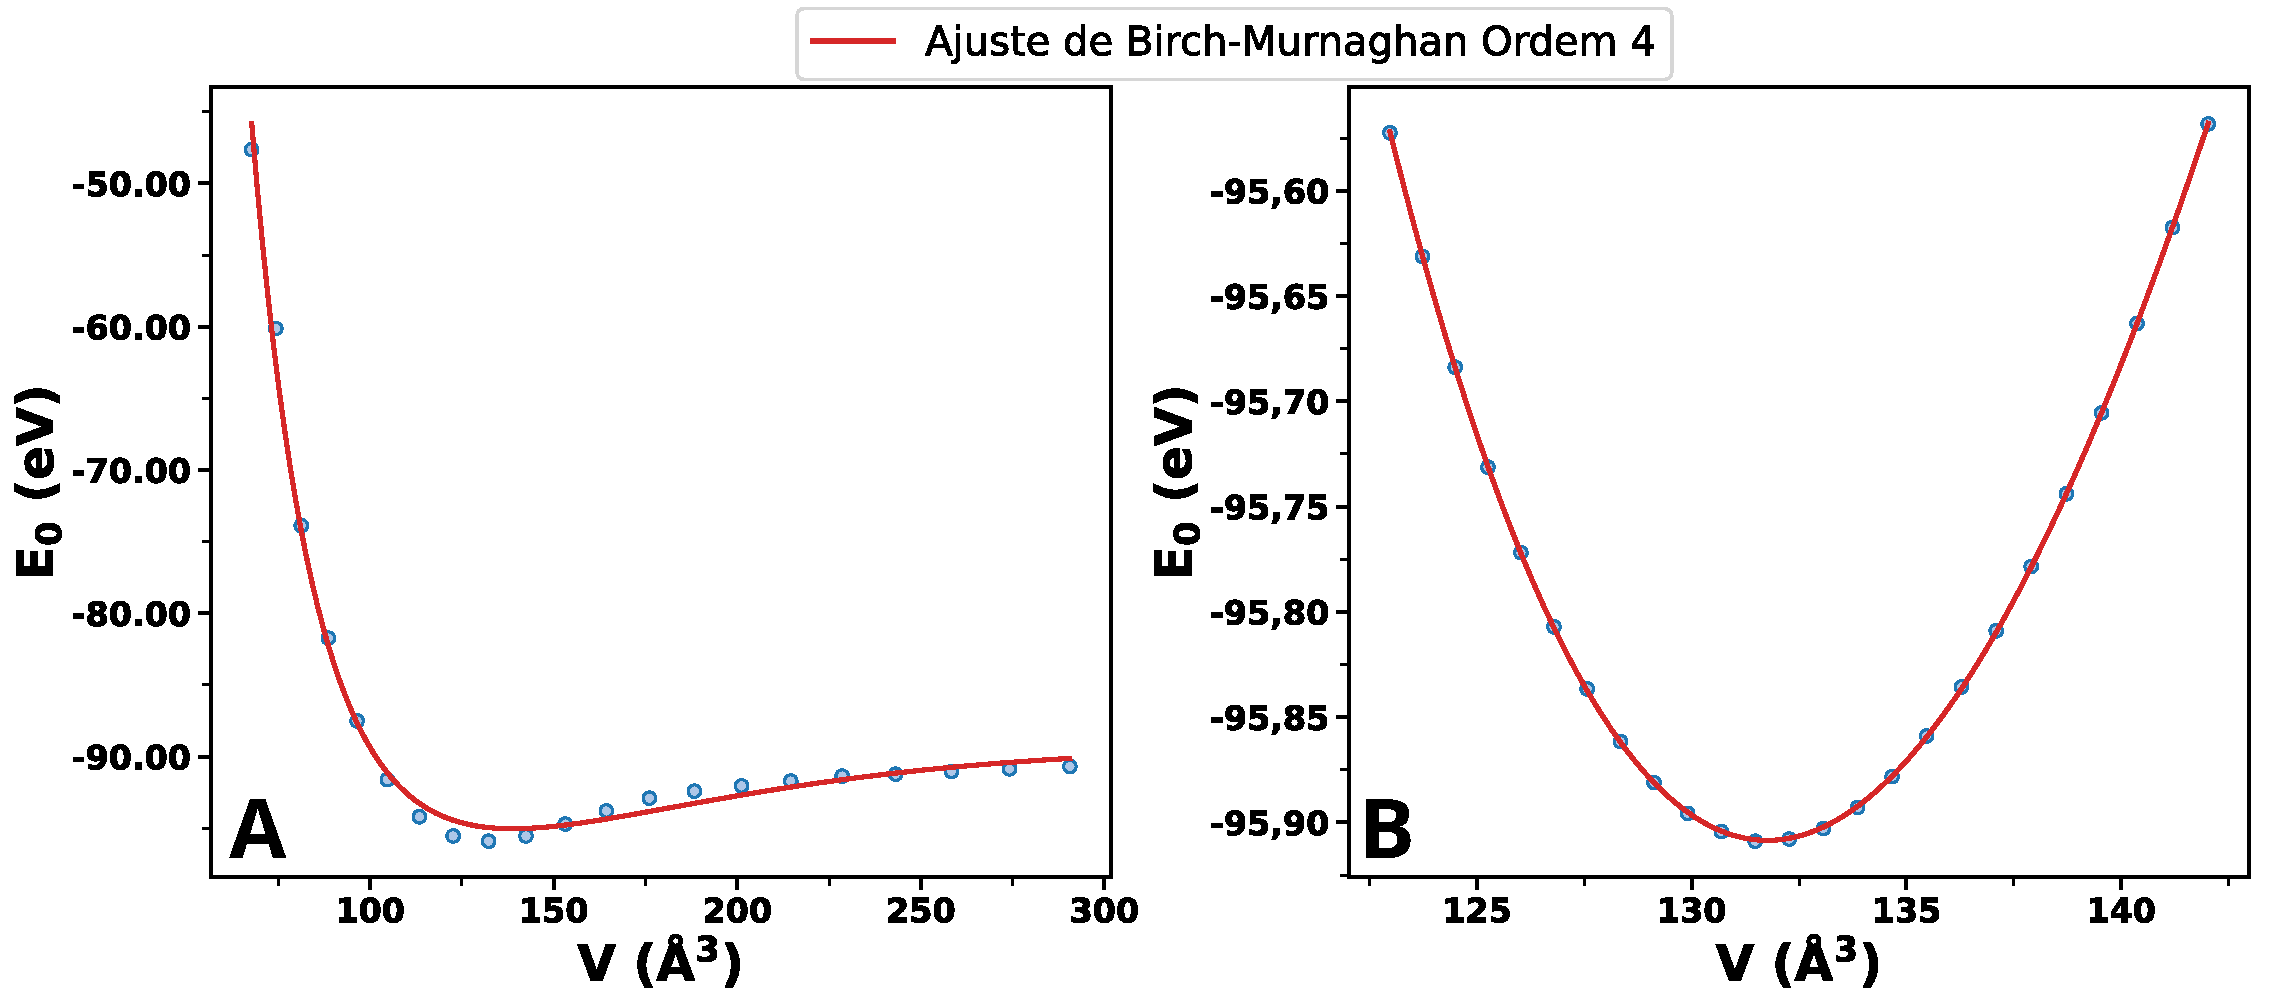
\includegraphics[width=1.0\textwidth]{figuras/graficos/curva_fit_birch.pdf}
    \fonte{Elaborada pelo autor.}
\end{figure}
\FloatBarrier

Os resultados preliminares expostos na Figura \ref{fig:curva_fit_birch}A foi observado que a energia total do sistema atinge um valor mínimo para no volume de 132,272 \AA$^3$ (fator de escala igual a 1,000). Ao realizar um estudo mais refinado com variações menores no fator de escala do parametro de rede próximo ao primeiro valor deminimo e fazendo um ajuste não linear utilizando a equação de Birch-Murnaghan foi obtida um volume mínimo de 131,480 \AA$^3$ (fator de escala igual a 0,998). Ao utilizar esse fator de escala de rede na estrutura do ZnWO$_4$ para obtenção da sua E$_0$ mínima comprovou-se que esse valor de fator de escala realmente corresponde ao valor mínimo de energia do sistema. Os parametros de rede obtido pela otimização de volume foram comparados com resultados experimentais e teóricos da literatura, para averiguar a validade dos resultados obtidos. A Tabela \ref{tab:parametros_de_rede_ZnWO4} os parametros de rede obtidos em comparativo com a literatura para o ZnWO$_4$.

\FloatBarrier
\begin{table}[!htbp]
\centering
\caption{Parametros de rede do ZnWO$_4$ frente ao literatura.}
\label{tab:parametros_de_rede_ZnWO4}
\begin{tabular}{lccc p{5cm}}
\hline
\textbf{Natureza do resultado} & \textbf{a} & \textbf{b} & \textbf{c} & \textbf{Referência}
\\ \hline
Calculado & 4,6674 & 5,7182 & 4,9364 & Presente trabalho \\
Calculado &  4.702 &  5.755 & 4.917 & Hoang (2018) \cite{hoang2018electronic} \\
Calculado & 4.736 & 5.746 & 4.937 & Zhang (2023) \cite{zhang2023effect} \\
Experimental & 4.6849 & 5.7172 & 4.9328 & Dkhilalli \textit{et. al.} (2018) \cite{dkhilalli2018structural} \\
Experimental &  4.691 & 5.720 &  4.925 & Yan \textit{et. al.} (2019) \cite{yan2019study} \\

\hline
\end{tabular}
\end{table}
\FloatBarrier

Ao comparar os resultados obtidos com a literatura foi observado um elevada similaridade entre os resultados. O que serve de indicativo de que o modelo construido apresnta boa representatividade estrutural do material.

Uma vez estabelecida o ENCUT, \textit{k-points}, funcional de troca correlação e parametros de rede que melhor descrevem do ZnWO$_4$ pode-se avançar para construção de possíveis terminações superfíciais do material bem como o estudo de suas estabilidade segundo a Termodinâmica Atomística de Primeiros Princípios \cite{reuter2005ab,rogal2006}.

\subsection{Construção das superfícies e estudo de estabilidade}
A partir da estrutura otimizada do ZnWO$_4$ foram construídas as superfícies de baixos índices de Miller (001), (010), (011), (100), (101) (110) e (111). \textcolor{red}{Essas superfícies foram escolhidas por serem as mais prováveis de serem expostas em cristais do material, conforme observado em estudos experimentais \cite{pereira2018znwo}}. Para cada orientação foram geradas diferentes terminações superficiais, de 15 \AA de espessura e com um vácuo de 15 \AA, totalizando 50 terminações. A Tabela \ref{tab:terminações_znwo4} apresenta o número terminações superficiais geradas para cada orientação e suas respectivas identificações.

\FloatBarrier
\begin{table}[!htbp]
\centering
\caption{Terminações superficiais geradas para cada orientação do ZnWO$_4$.}
\label{tab:terminações_znwo4}
\begin{tabular}{lcc}
\hline
\textbf{Orientação} & \textbf{Identificação} & \textbf{Número de Terminações}
\\ \hline
(001) & ST-A & 5 \\
(010) & ST-B & 8 \\
(011) & ST-C & 12 \\
(100) & ST-D & 6 \\
(101) & ST-E & 3 \\
(110) & ST-F & 8 \\
(111) & ST-G & 8 \\
\hline
\end{tabular}
\end{table}
\FloatBarrier

Os \textit{slabs} referentes as terminações geradas para cada superficies tiveram sua estabilidade avaliada por meio do calculo de energia livre de superfície ($\gamma$) segundo a Equação \ref{eq:gibbs_superficie_final}, com o auxílio da plataforma de automatização de calculos PS-TEROS. A partir dessa equação é possível avaliar a estabilidade de diferentes terminações de forma comparativa de duas maneiras. Primeiro traçando um diagrama de energia em que é estabelecida uma condição de potencial químico do cátion metálico modificador de rede (neste caso definindo como zero) e calculando a energia livre de superfície em função do potencial químico do oxigênio, permitindo assim identificar qual terminação é mais estável para uma determinada condição de ambiente químico. A segunda maneira é traçando um diagrama de estabilidade das terminações em que varia-se tanto o potencial químico do oxigênio quanto o do cátion metálico modificador da rede, permitindo assim identificar quais terminações são termodinamicamente mais estáveis sob diferentes condições de ambiente químico. Também é posssível relacionar a temperatura e pressão do ambiente químico com os potenciais químicos do oxigênio (Equação \ref{eq:delta_mu_o_temp_press}), permitindo assim estabelecer condições experimentais para a obtenção de determinadas terminações superficiais.



\subsubsection{Estudo de estabilidade superfície (001)}

Para a orientação (001) foram geradas 5 terminações superficiais diferentes, identificadas como ST-A1 a ST-A5. A Figura \ref{fig:znwo4_superficie_001} apresenta as estruturas das diferentes terminações superficiais geradas para essa orientação, antes e após a relaxação das estruturas, bem como seus defeitos estruturais.

\FloatBarrier
\begin{figure}[!htbp]
    \caption{Estruturas das diferentes terminações superficiais (001) do ZnWO$_4$: (A) ST-A1, (B) ST-A2, (C) ST-A3, (D) ST-A4 e (E) ST-A5, antes e após a relaxação das estruturas.}
    \label{fig:znwo4_superficie_001}
    \centering
    
\includegraphics[width=0.50\textwidth]{figuras/imagens/exemplo.jpg}
    \fonte{Elaborada pelo autor.}
\end{figure}
\FloatBarrier

A partir dos E$_0$ obtidos para cada terminação superficial, foi possível $\gamma$ em função de $\Delta \mu_O$ e também foi possível gerar o diagrama de superfície que relaciona o $\mu_O$ com $\Delta \mu_Zn$. Os resultados desses cálculos estão apresentados na Figura \ref{fig:energia_superficie_001}.

\FloatBarrier
\begin{figure}[!htbp]
    \caption{(A) $\gamma$ em função de $\Delta \mu_O$ para as diferentes terminações superficiais (001) do ZnWO$_4$. (B) Diagrama de estabilidade das terminações superficiais (001) em função dos potenciais químicos do oxigênio $\Delta \mu_O$ e $\Delta \mu_{Zn}$. (C) Relação de T para diferentes $\Delta \mu_O$ e pressões parciais de O$_2$.}
    \label{fig:energia_superficie_001}
    \centering
    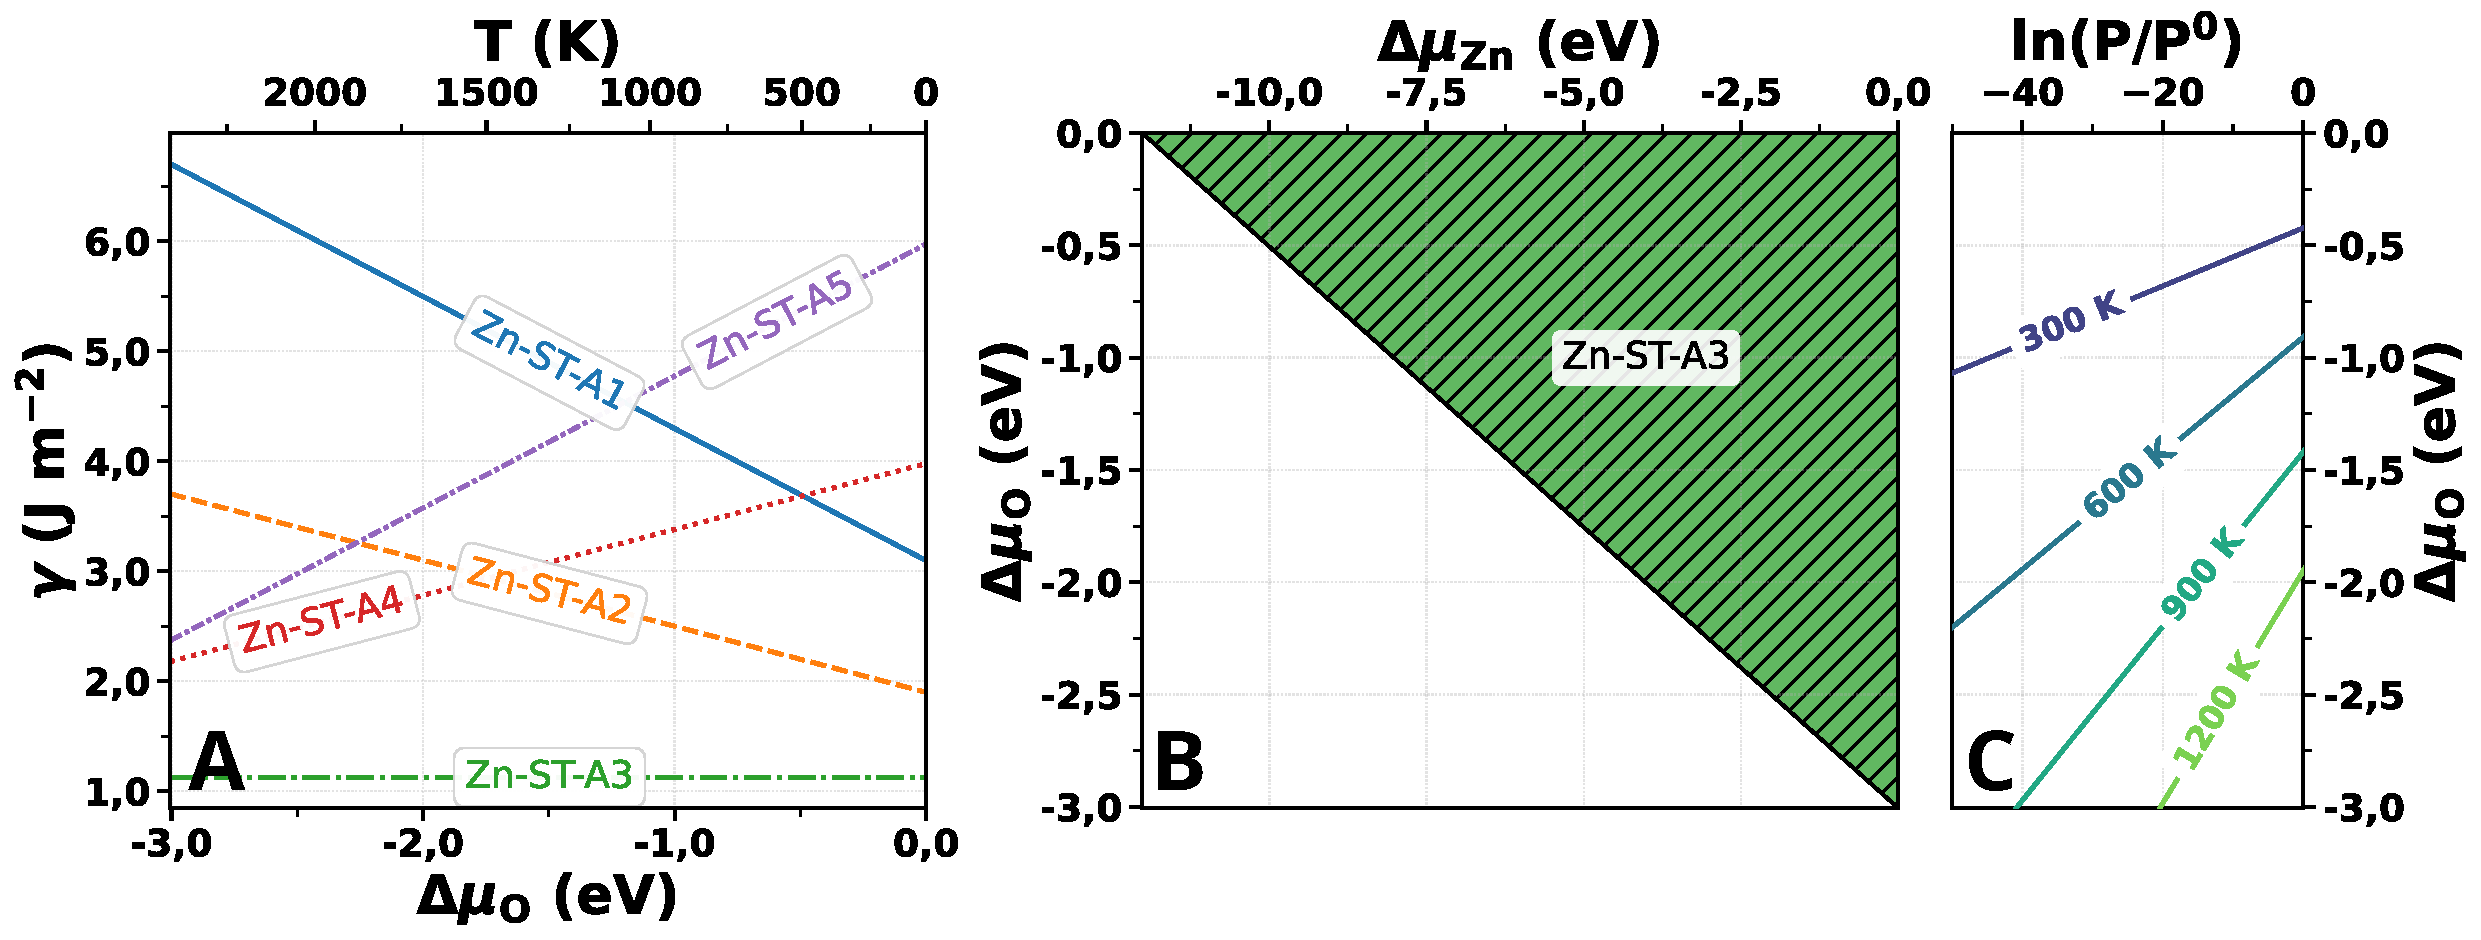
\includegraphics[width=1.0\textwidth]{figuras/graficos/energia_superficie_001.pdf}
    \fonte{Elaborada pelo autor.}
\end{figure}
\FloatBarrier

\subsubsection{Estudo de estabilidade superfície (010)}
Para a orientação (010) foram geradas 8 terminações superficiais diferentes, identificadas como ST-B1 a ST-B8. A Figura \ref{fig:znwo4_superficie_010} apresenta as estruturas das diferentes terminações superficiais geradas para essa orientação, antes e após a relaxação das estruturas, bem como seus defeitos estruturais.

\FloatBarrier
\begin{figure}[!htbp]
    \caption{Estruturas das diferentes terminações superficiais (010) do ZnWO$_4$: (A) ST-B1, (B) ST-B2, (C) ST-B3, (D) ST-B4, (E) ST-B5, (F) ST-B6, (G) ST-B7 e (H) ST-B8, antes e após a relaxação das estruturas.}
    \label{fig:znwo4_superficie_010}
    \centering
    
\includegraphics[width=0.50\textwidth]{figuras/imagens/exemplo.jpg}
    \fonte{Elaborada pelo autor.}
\end{figure}
\FloatBarrier

A partir dos E$_0$ obtidos para cada terminação superficial, foi possível calcular $\gamma$ em função de $\Delta \mu_O$. Também foi possível gerar o diagrama de superfície que relaciona o $\Delta \mu_O$ com $\Delta \mu_{Zn}$. Os resultados desses cálculos estão apresentados na Figura \ref{fig:energia_superficie_010}.

\FloatBarrier
\begin{figure}[!htbp]
    \caption{(A) $\gamma$ em função de $\Delta \mu_O$ para as diferentes terminações superficiais (010) do ZnWO$_4$ (B) Diagrama de estabilidade das terminações superficiais (010) em função de $\Delta \mu_O$ e $\Delta \mu_{Zn}$. (C) Relação de T para diferentes $\Delta \mu_O$ e pressões parciais de O$_2$.}
    \label{fig:energia_superficie_010}
    \centering
    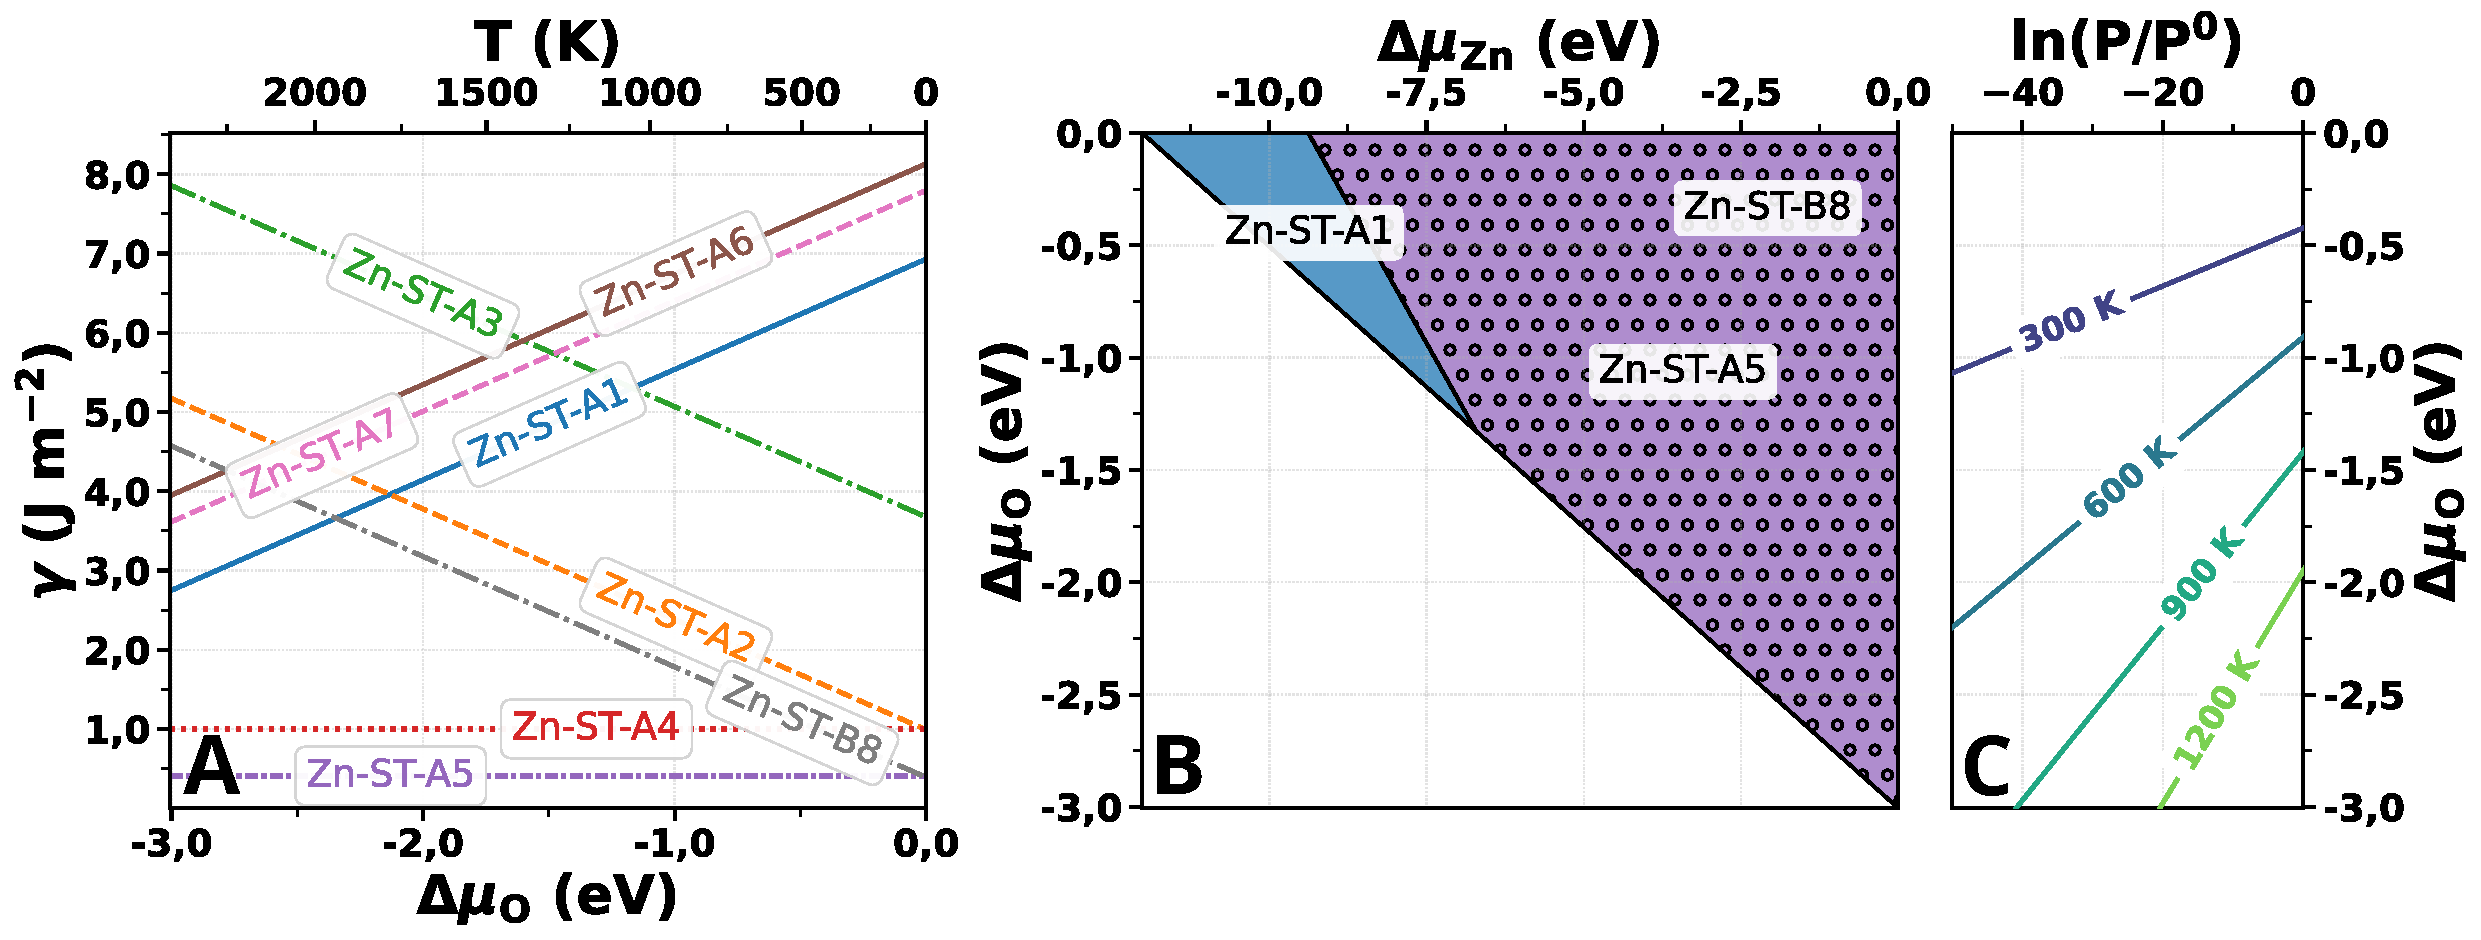
\includegraphics[width=1.0\textwidth]{figuras/graficos/energia_superficie_010.pdf}
    \fonte{Elaborada pelo autor.}
\end{figure}
\FloatBarrier

\subsubsection{Estudo de estabilidade superfície (011)}
Para a orientação (011) foram geradas 12 terminações superficiais diferentes, identificadas como ST-C1 a ST-C12. A Figura \ref{fig:znwo4_superficie_011} apresenta as estruturas das diferentes terminações superficiais geradas para essa orientação, antes e após a relaxação das estruturas, bem como seus defeitos estruturais.

\FloatBarrier
\begin{figure}[!htbp]
    \caption{Estruturas das diferentes terminações superficiais (011) do ZnWO$_4$: (A) ST-C1, (B) ST-C2, (C) ST-C3, (D) ST-C4, (E) ST-C5, (F) ST-C6, (G) ST-C7, (H) ST-C8, (I) ST-C9, (J) ST-C10, (K) ST-C11 e (L) ST-C12, antes e após a relaxação das estruturas.}
    \label{fig:znwo4_superficie_011}
    \centering
    
\includegraphics[width=0.50\textwidth]{figuras/imagens/exemplo.jpg}
    \fonte{Elaborada pelo autor.}
\end{figure}
\FloatBarrier


\subsubsection{Estudo de estabilidade superfície (100)}
Para a orientação (100) foram geradas 6 terminações superficiais diferentes, identificadas como ST-D1 a ST-D6. A Figura \ref{fig:znwo4_superficie_100} apresenta as estruturas das diferentes terminações superficiais geradas para essa orientação, antes e após a relaxação das estruturas, bem como seus defeitos estruturais.

\FloatBarrier
\begin{figure}[!htbp]
    \caption{Estruturas das diferentes terminações superficiais (100) do ZnWO$_4$: (A) ST-D1, (B) ST-D2, (C) ST-D3, (D) ST-D4, (E) ST-D5 e (F) ST-D6, antes e após a relaxação das estruturas, bem como seus defeitos estruturais.}
    \label{fig:znwo4_superficie_100}
    \centering
    
\includegraphics[width=0.50\textwidth]{figuras/imagens/exemplo.jpg}
    \fonte{Elaborada pelo autor.}
\end{figure}
\FloatBarrier

A partir dos E$_0$ obtidos para cada terminação superficial, foi possível calcular $\gamma$ em função de $\Delta \mu_O$. Também foi possível gerar o diagrama de superfície que relaciona o $\Delta \mu_O$ com $\Delta \mu_{Zn}$. Os resultados desses cálculos estão apresentados na Figura \ref{fig:energia_superficie_100}.

\FloatBarrier
\begin{figure}[!htbp]
    \caption{(A) $\gamma$ em função de $\Delta \mu_O$ para as diferentes terminações superficiais (100) do ZnWO$_4$ (B) Diagrama de estabilidade das terminações superficiais (100) em função de $\Delta \mu_O$ e $\Delta \mu_{Zn}$. (C) Relação de T para diferentes $\Delta \mu_O$ e pressões parciais de O$_2$.}
    \label{fig:energia_superficie_100}
    \centering
    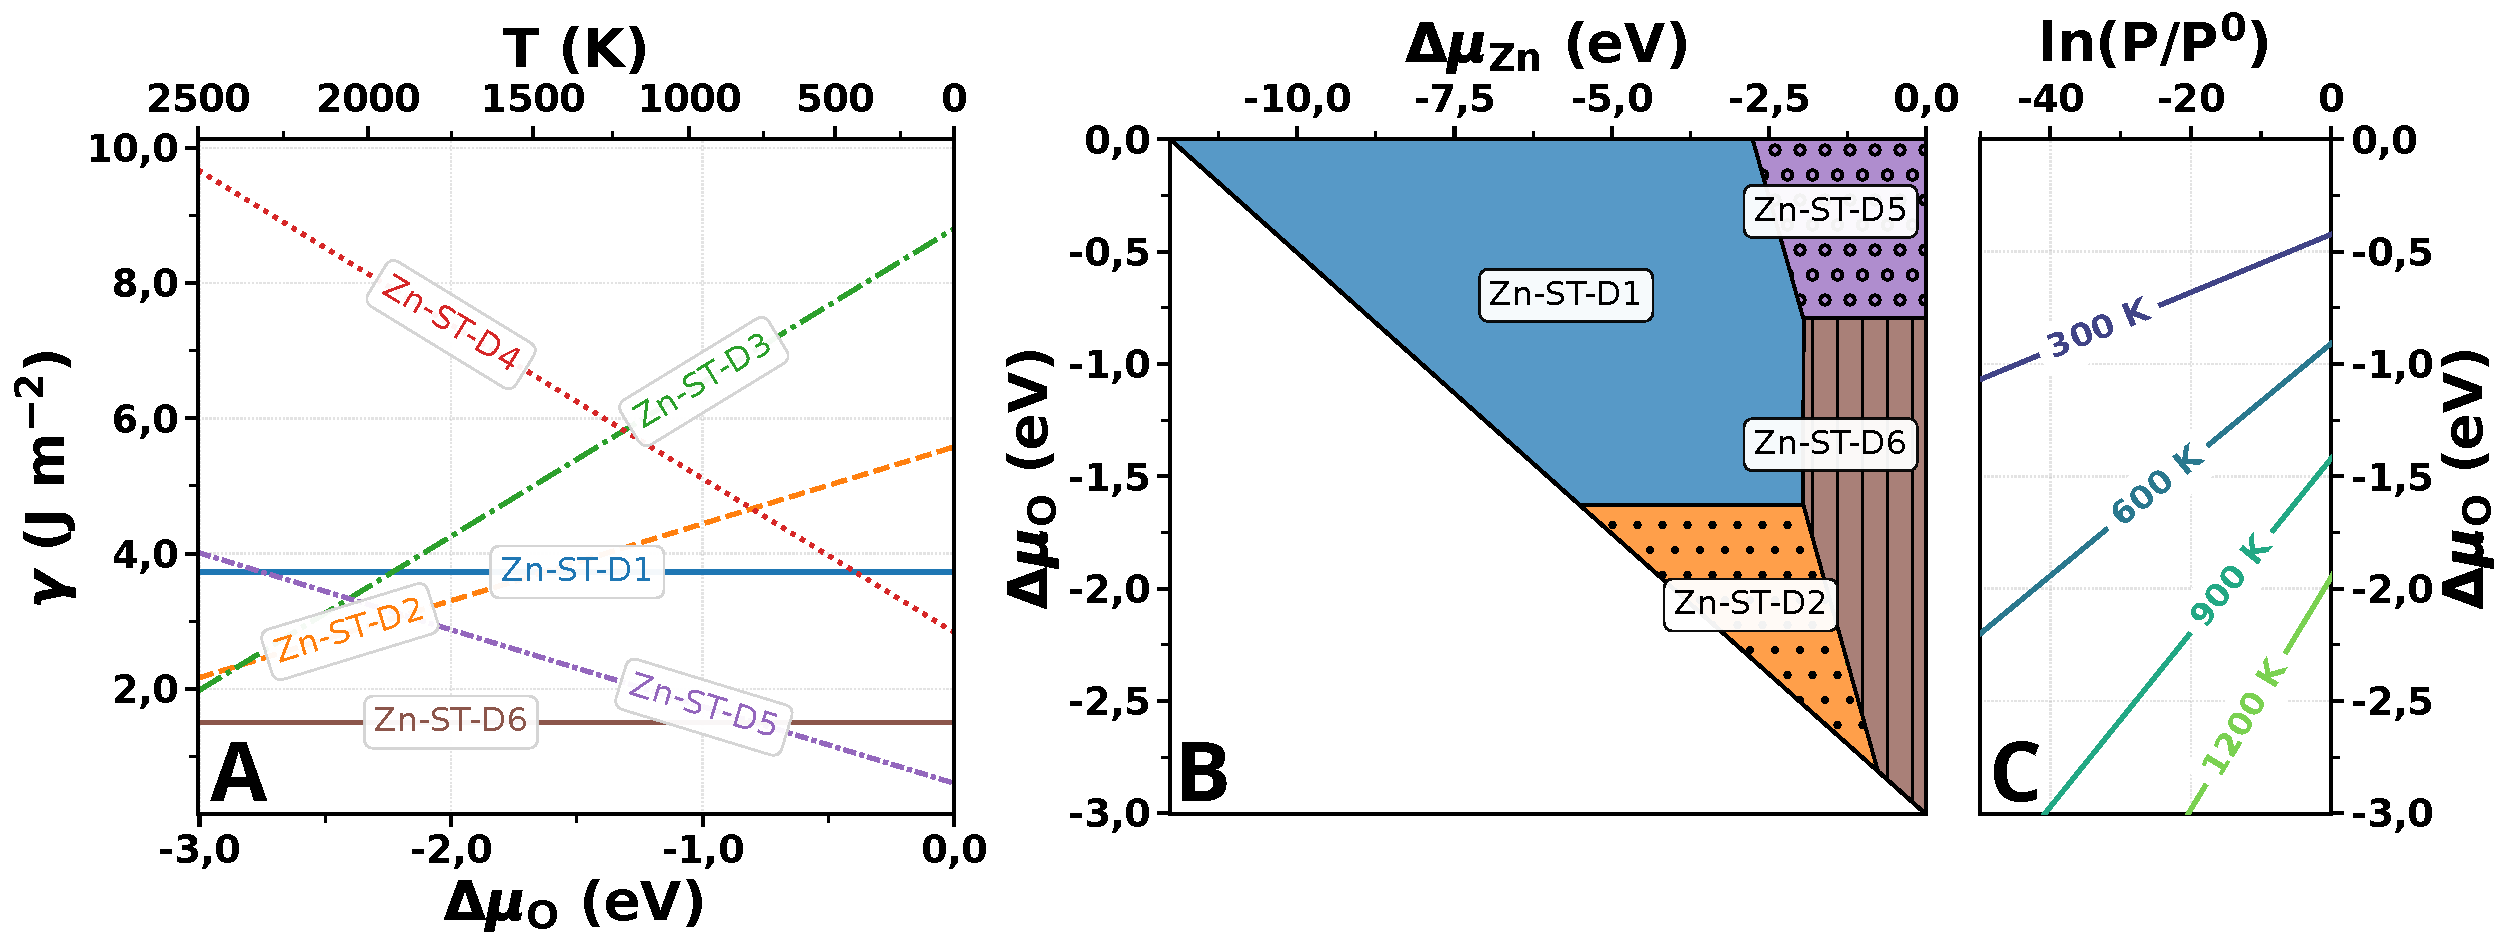
\includegraphics[width=1.0\textwidth]{figuras/graficos/energia_superficie_100.pdf}
    \fonte{Elaborada pelo autor.}
\end{figure}
\FloatBarrier

\subsubsection{Estudo de estabilidade superfície (101)}
Para a orientação (101) foram geradas 3 terminações superficiais diferentes, identificadas como ST-E1, ST-E2 e ST-E3. A Figura \ref{fig:znwo4_superficie_101} apresenta as estruturas das diferentes terminações superficiais geradas para essa orientação, antes e após a relaxação das estruturas, bem como seus defeitos estruturais.

\FloatBarrier
\begin{figure}[!htbp]
    \caption{Estruturas das diferentes terminações superficiais (101) do ZnWO$_4$: (A) ST-E1, (B) ST-E2 e (C) ST-E3, antes e após a relaxação das estruturas.}
    \label{fig:znwo4_superficie_101}
    \centering
    
\includegraphics[width=0.50\textwidth]{figuras/imagens/exemplo.jpg}
    \fonte{Elaborada pelo autor.}
\end{figure}
\FloatBarrier

A partir dos E$_0$ obtidos para cada terminação superficial, foi possível calcular $\gamma$ em função de $\Delta \mu_O$. Também foi possível gerar o diagrama de superfície que relaciona o $\Delta \mu_O$ com $\Delta \mu_{Zn}$. Os resultados desses cálculos estão apresentados na Figura \ref{fig:energia_superficie_101}.

\FloatBarrier
\begin{figure}[!htbp]
    \caption{(A) $\gamma$ em função de $\Delta \mu_O$ para as diferentes terminações superficiais (101) do ZnWO$_4$ (B) Diagrama de estabilidade das terminações superficiais (101) em função de $\Delta \mu_O$ e $\Delta \mu_{Zn}$. (C) Relação de T para diferentes $\Delta \mu_O$ e pressões parciais de O$_2$.}
    \label{fig:energia_superficie_101}
    \centering
    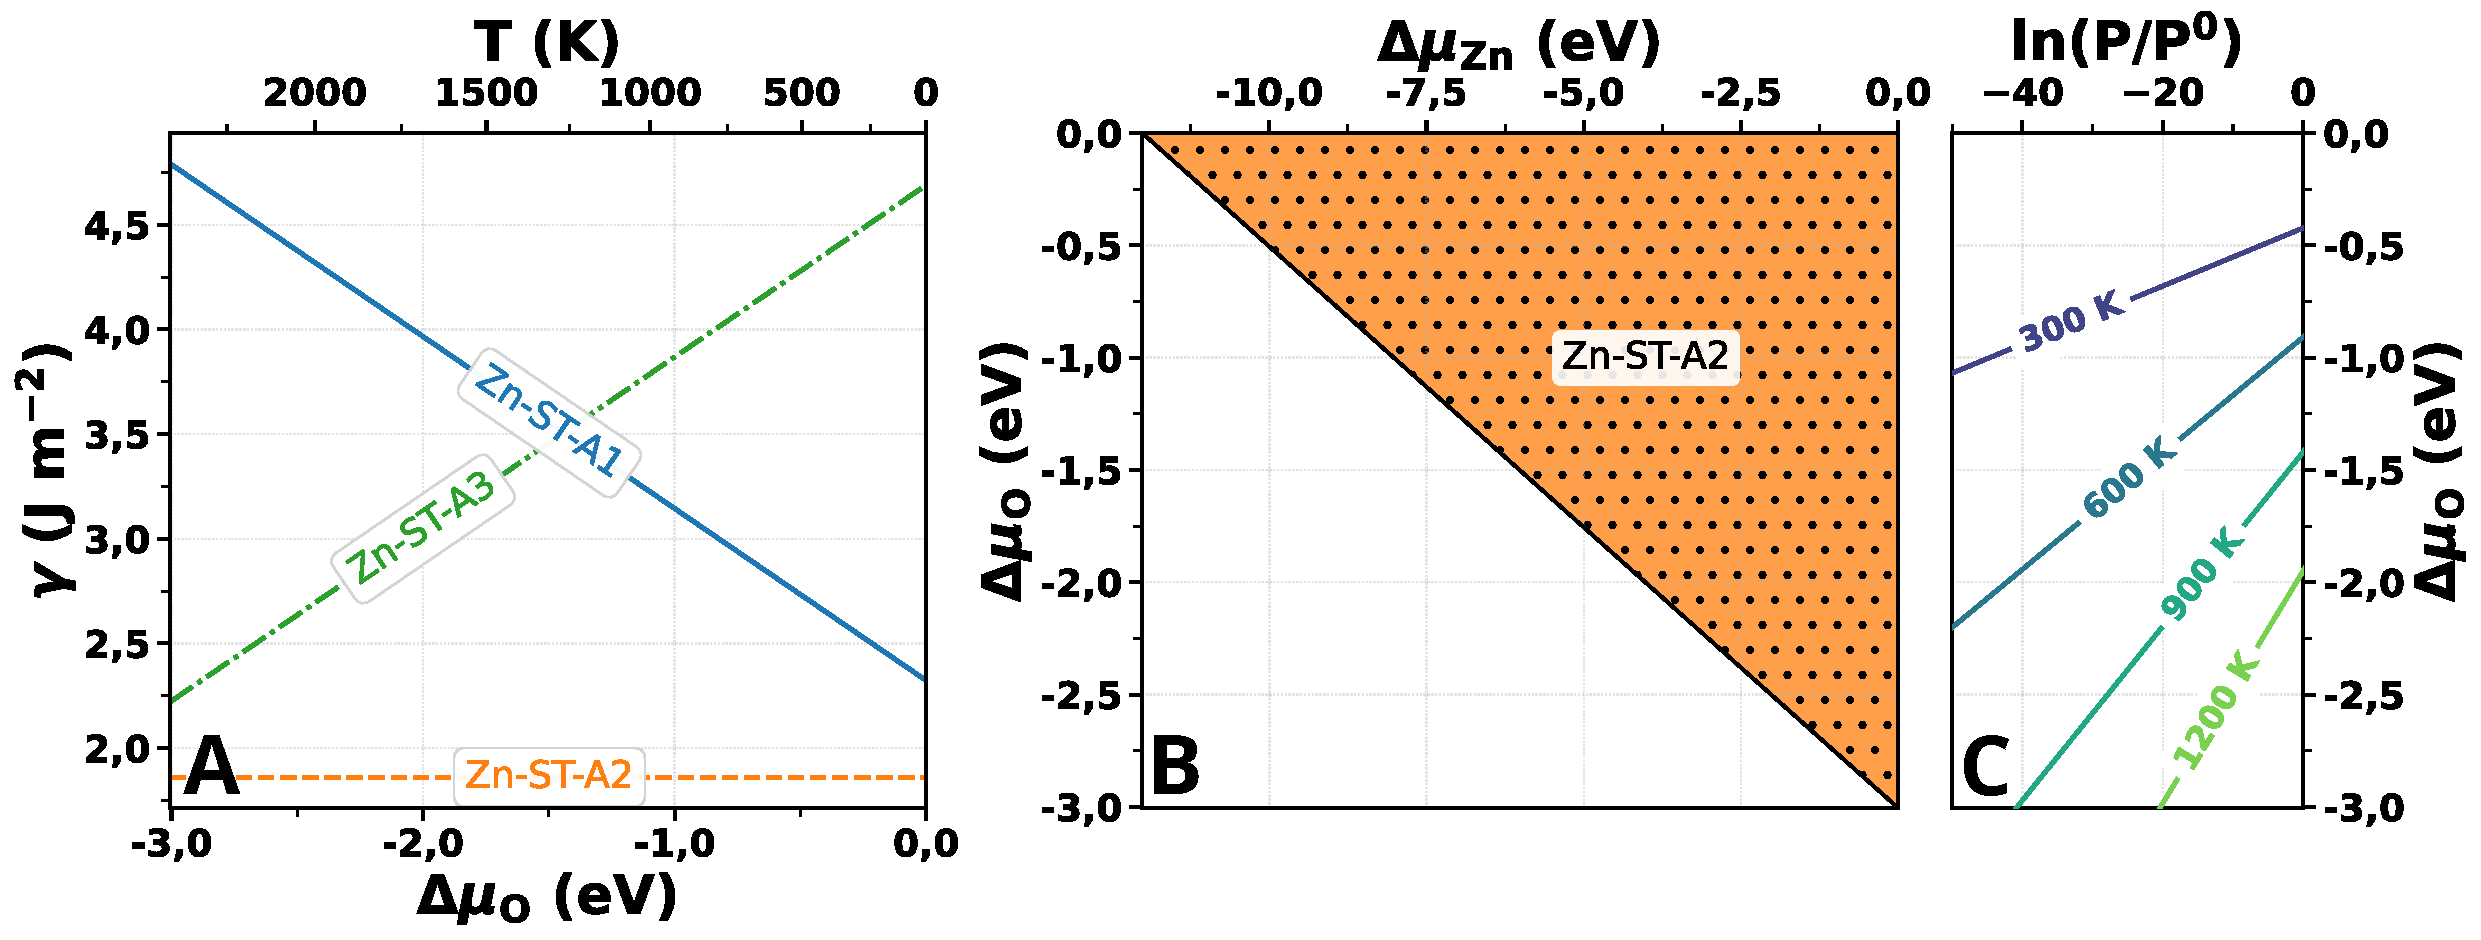
\includegraphics[width=1.0\textwidth]{figuras/graficos/energia_superficie_101.pdf}
    \fonte{Elaborada pelo autor.}
\end{figure}
\FloatBarrier

\subsubsection{Estudo de estabilidade superfície (110)}
Para a orientação (110) foram geradas 8 terminações superficiais diferentes, identificadas como ST-F1 a ST-F8. A Figura \ref{fig:znwo4_superficie_110} apresenta as estruturas das diferentes terminações superficiais geradas para essa orientação, antes e após a relaxação das estruturas, bem como seus defeitos estruturais.

\FloatBarrier
\begin{figure}[!htbp]
    \caption{Estruturas das diferentes terminações superficiais (110) do ZnWO$_4$: (A) ST-F1, (B) ST-F2, (C) ST-F3, (D) ST-F4, (E) ST-F5, (F) ST-F6, (G) ST-F7 e (H) ST-F8, antes e após a relaxação das estruturas.}
    \label{fig:znwo4_superficie_110}
    \centering
    
\includegraphics[width=0.50\textwidth]{figuras/imagens/exemplo.jpg}
    \fonte{Elaborada pelo autor.}
\end{figure}
\FloatBarrier

A partir dos E$_0$ obtidos para cada terminação superficial, foi possível calcular $\gamma$ em função de $\Delta \mu_O$. Também foi possível gerar o diagrama de superfície que relaciona o $\Delta \mu_O$ com $\Delta \mu_{Zn}$. Os resultados desses cálculos estão apresentados na Figura \ref{fig:energia_superficie_110}.

\FloatBarrier
\begin{figure}[!htbp]
    \caption{(A) $\gamma$ em função de $\Delta \mu_O$ para as diferentes terminações superficiais (110) do ZnWO$_4$ (B) Diagrama de estabilidade das terminações superficiais (110) em função de $\Delta \mu_O$ e $\Delta \mu_{Zn}$. (C) Relação de T para diferentes $\Delta \mu_O$ e pressões parciais de O$_2$.}
    \label{fig:energia_superficie_110}
    \centering
    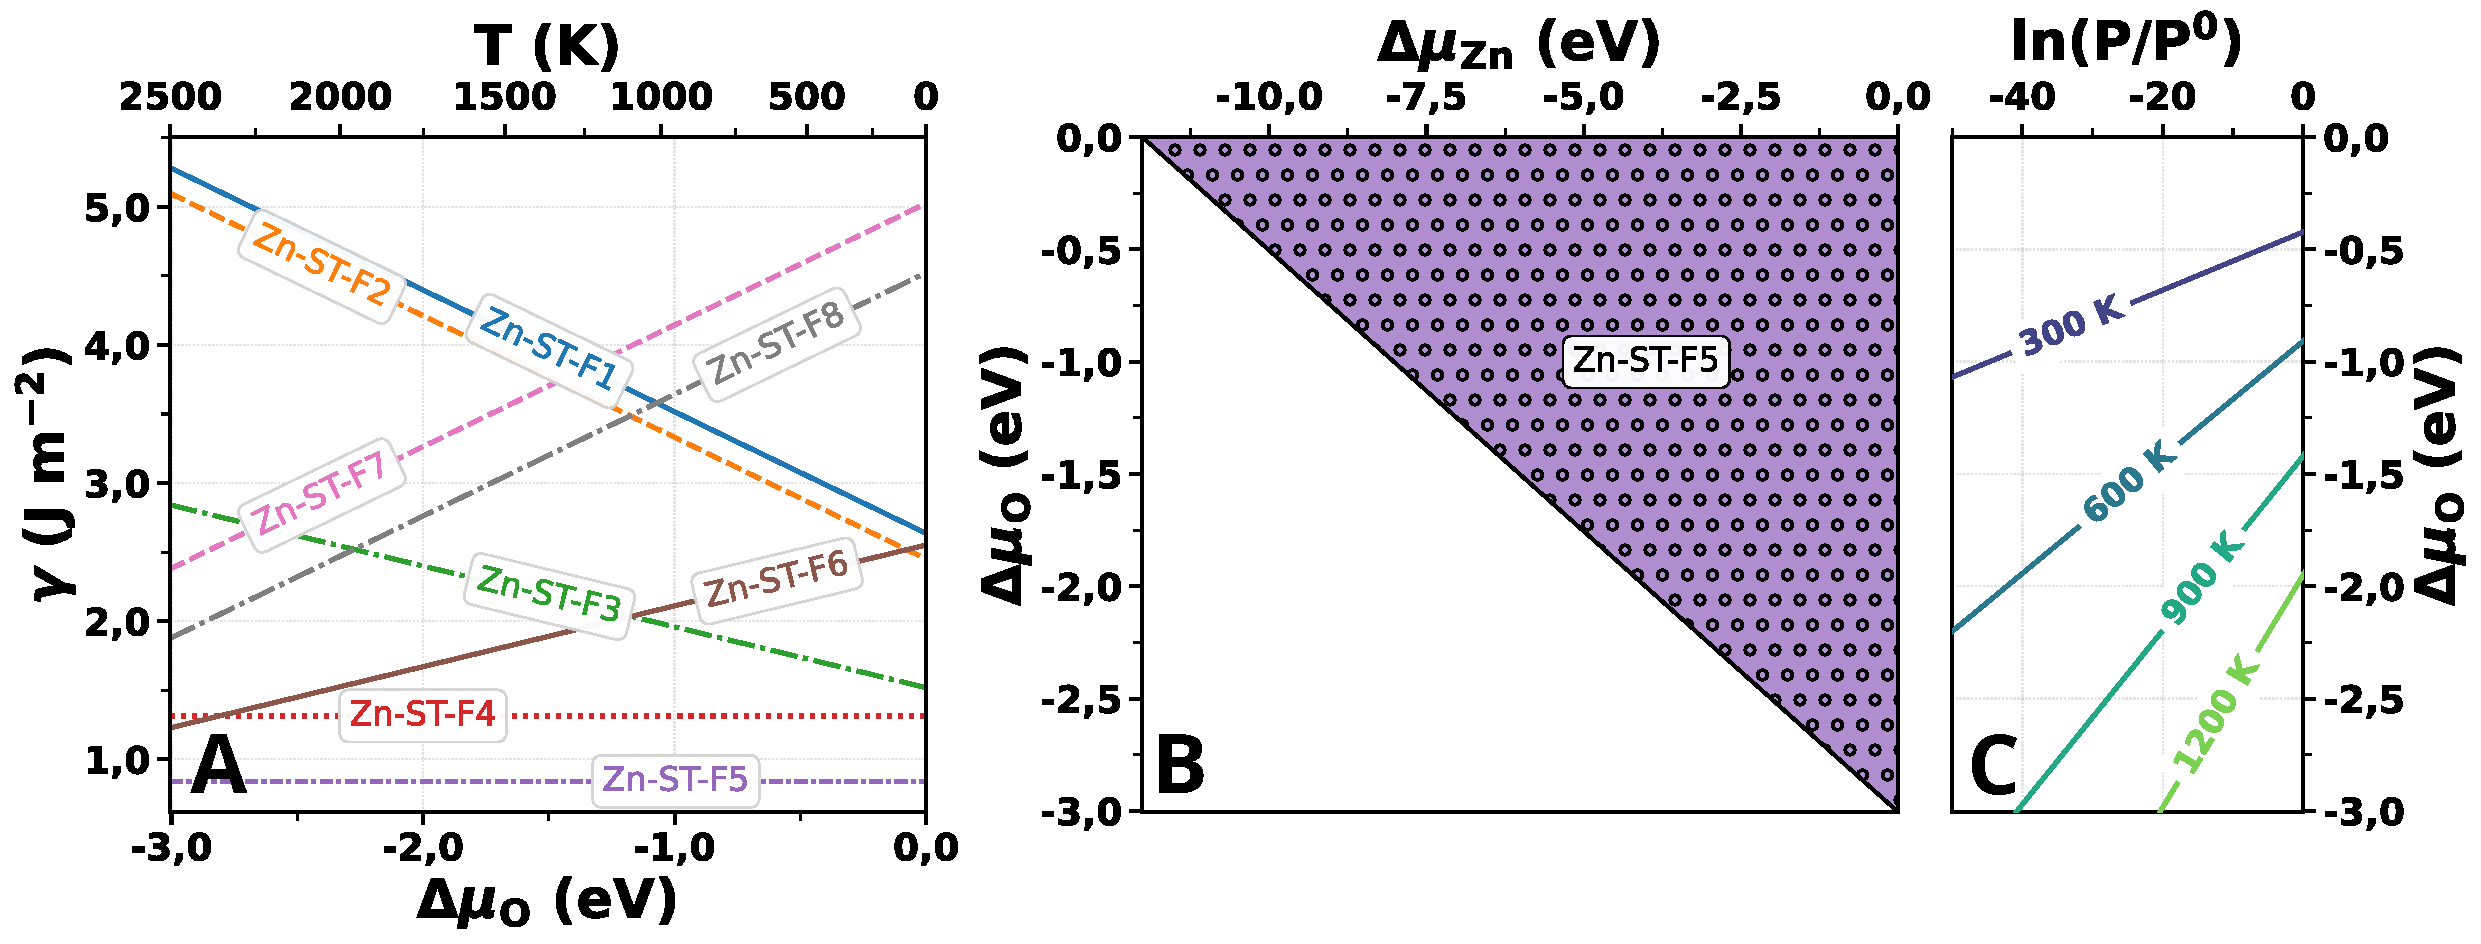
\includegraphics[width=1.0\textwidth]{figuras/graficos/energia_superficie_110.pdf}
    \fonte{Elaborada pelo autor.}
\end{figure}
\FloatBarrier

\subsubsection{Estudo de estabilidade superfície (111)}
Por fim para a orientação (111) foram geradas 8 terminações superficiais diferentes, identificadas como ST-G1 a ST-G8. A Figura \ref{fig:znwo4_superficie_111} apresenta as estruturas das diferentes terminações superficiais geradas para essa orientação, antes e após a relaxação das estruturas, bem como seus defeitos estruturais.

\FloatBarrier
\begin{figure}[!htbp]
    \caption{Estruturas das diferentes terminações superficiais (111) do ZnWO$_4$: (A) ST-G1, (B) ST-G2, (C) ST-G3, (D) ST-G4, (E) ST-G5, (F) ST-G6, (G) ST-G7 e (H) ST-G8, antes e após a relaxação das estruturas.}
    \label{fig:znwo4_superficie_111}
    \centering
    
\includegraphics[width=0.50\textwidth]{figuras/imagens/exemplo.jpg}
    \fonte{Elaborada pelo autor.}
\end{figure}
\FloatBarrier

% Inclua figuras e tabelas conforme necessário.
